\documentclass[openany]{article}
\usepackage[a4paper,margin=1in,bottom=1.5in]{geometry}
\usepackage[english]{babel}
\usepackage{tikz}
\usepackage{graphicx}
\usepackage[export]{adjustbox}
\usepackage{fancyhdr}
\usepackage{array} % allow elements of tabular environment to have vertical alignment, e.g., center alignment.

% Configure header in 'titlepage'
\pagestyle{fancy}
\lhead{
\includegraphics[width=4.5cm]{logo_cnpem}}
\rhead{
\includegraphics[width=4cm]{logo_lnls}}
\renewcommand{\headrulewidth}{0pt}
\setlength{\headheight}{52pt}
% Clean footer
\fancyfoot{}

% increase table height factor a little bit (taller cells)
\renewcommand{\arraystretch}{1.5}

%==== Begin DOCUMENT ====
\begin{document}

%--- Begin title page ---
\begin{titlepage}

% Add header to this page
\thispagestyle{fancy}

% Center elements
\begin{center}

\topskip0pt
\vspace*{\fill}
\textbf{\Huge SOE Hardware Manual}\\[20pt]
\textbf{\Huge Version 1.0}\\[20pt]
\textbf{\Huge February/2017}
\vspace*{\fill}

\vfill
\textbf{Beam Diagnostics Group (DIG)}\\[5pt]
\textbf{Brazilian Synchrotron Light Laboratory (LNLS)}\\[5pt]
\textbf{Brazilian Center for Research in Energy and Materials (CNPEM)}
\end{center}

\end{titlepage}
%--- End of title page ---

\newpage
\pagestyle{plain}

%--- About this manual ---
\paragraph{}{\Large\bfseries About this manual}

\paragraph{} This manual is intended for people who need information about the SOE hardware. Information about the timing system structure and operation, firmware, or software can be found in the corresponding manuals.

%--- Table of contents ---
\tableofcontents

\newpage
%--- Section: Hardware Specification ---
\section{Hardware Specification}

\par SOE is a standalone module. \\ 18 - 36V DC power supply.

% STD-SOE figure
\begin{figure}[!h]
\caption{SOE}
\label{fig:soe}
\centering
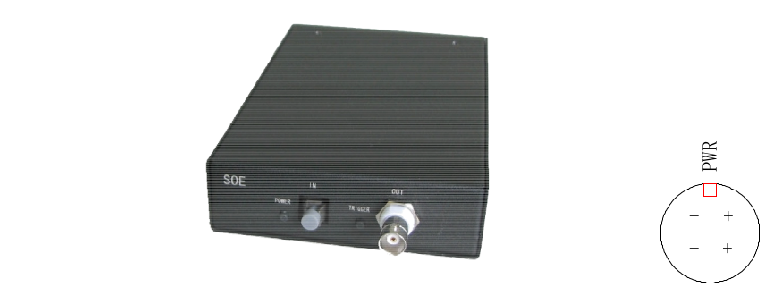
\includegraphics[width=0.7\textwidth]{soe-image}
\end{figure}

	% Specification table - Connectors - front panel
	\begin{table}[!h]
	  \centering
	  \caption{SOE front panel connectors}
	  \label{tab:front-panel-connectors}
	  \begin{tabular}{| m{3.5cm} m{4.0cm} m{7.0cm} |}
	    \hline
	    \bfseries Connector & \bfseries Type & \bfseries Description / Specification \\ \hline
	    IN & HFBR-4531/4532 & Optical Input (Agilent HFBR-2528) \\ \hline
	    OUT & BNC & Outputs (5.0V TTL level) \\ \hline
	  \end{tabular}
	\end{table}

	% Specification table - LEDs - front panel
	\begin{table}[!h]
	  \centering
	  \caption{SOE front panel leds}
	  \label{tab:front-panel-leds}
	  \begin{tabular}{| m{3.5cm} m{4.0cm} m{7.0cm} |}
	    \hline
	    \bfseries LED & \bfseries Type & \bfseries Description / Specification \\ \hline
	    PWR & Green LED & Power on \\ \hline
	    TRIGGER & Yellow LED & (Blink) Trigger output \\ \hline
	  \end{tabular}
	\end{table}

	% Specification table - Connectors - rear panel
	\begin{table}[!h]
	  \centering
	  \caption{SOE rear panel connectors}
	  \label{tab:rear-panel-connectors}
	  \begin{tabular}{| m{3.5cm} m{4.0cm} m{7.0cm} |}
	    \hline
	    \bfseries Connector & \bfseries Type & \bfseries Description / Specification \\ \hline
	    PWR & LEMO.EXG.1B.304.HLN & \begin{tabular}{@{}m{6cm}@{}}
					Power supply \\
			    		18 - 36V DC
					\end{tabular} \\ \hline
	  \end{tabular}
	\end{table}

%--- Section: SOE Hardware ---
\section{SOE Hardware Functions}

	\paragraph{} The SOE is a standalone Optical to Electrical converter used for converting the Timing System triggers. The module has 1 Plastic Optical Fiber input (IN) in the front panel. The input signal is converted to a 5V TTL level electrical signal available in the BNC OUT output.

\end{document}
\grid
